\section{Вспомогательная структура данных для хранения карты высот}

Введём структуру данных HeightHandler: она хранит для поверхности паллеты поле текущих высот и вызывается при каждом размещении коробки.

Интерфейс включает четыре операции. Запрос $\mathtt{get\_h}(x_1, y_1, x_2, y_2)$ даёт максимум высоты в прямоугольнике $[x_1, x_2] \times [y_1, y_2]$. Запрос $\mathtt{get\_area}(x_1, y_1, x_2, y_2)$ --- площадь участка на этой максимальной высоте внутри того же прямоугольника; по ней оценивается опора коробки. Операция $\mathtt{add\_rect}(x_1, y_1, x_2, y_2, h)$ вносит новый прямоугольник высоты $h$ и обновляет карту. Наконец, $\mathtt{get\_dots}(\mathit{box})$ возвращает кандидатов в позиции размещения для коробки заданных габаритов.

Операция $\mathtt{get\_dots}$ формирует множество потенциальных позиций на основе углов уже размещённых прямоугольников. Такой подход позволяет сократить пространство поиска с $O(W \times L)$ до $O(n)$, где $W$ и $L$ --- размеры паллеты, а $n$ --- количество уже уложенных коробок.

В рамках работы были исследованы пять различных реализаций структуры HeightHandler, различающихся алгоритмическими подходами: наивная реализация Baseline, оптимизированный список Rects, плотная двумерная сетка Grid, двумерное дерево отрезков SegTree и квадродерево Quadtree.

Реализация Baseline представляет собой простейший вариант, в котором все добавленные прямоугольники хранятся в массиве. При выполнении запросов $\mathtt{get\_h}$ и $\mathtt{get\_area}$ производится полный перебор всех элементов массива. Вычислительная сложность операций $\mathtt{get\_h}$ и $\mathtt{get\_area}$ составляет $O(n)$, тогда как операция $\mathtt{add\_rect}$ выполняется за константное время $O(1)$. Корректность данной реализации гарантируется свойством задачи паллетизации: прямоугольники добавляются послойно, поэтому новый прямоугольник всегда имеет высоту строго большую, чем существующие прямоугольники в той же области.

Реализация Rects является оптимизированной версией Baseline, в которой прямоугольники поддерживаются отсортированными по убыванию высоты. Такая организация данных позволяет завершить поиск максимума при первом обнаружении пересечения с запрашиваемой областью. Вычислительная сложность операций $\mathtt{get\_h}$ и $\mathtt{get\_area}$ в худшем случае остаётся $O(n)$, однако на практике наблюдается существенное ускорение за счёт раннего выхода из цикла. Сложность операции $\mathtt{add\_rect}$ составляет $O(n)$ вследствие необходимости поддержания упорядоченности.

Реализация Grid разбивает паллету на ячейки фиксированного размера $10 \times 10$ мм. В каждой ячейке хранится максимальная высота. Для стандартной паллеты размером $1200 \times 800$ мм структура содержит $120 \times 80 = 9600$ ячеек. Вычислительная сложность всех операций составляет $O(k)$, где $k$ --- количество ячеек, затрагиваемых запросом. Недостатком данной реализации является значительный объём используемой памяти и медленное обновление при добавлении крупных прямоугольников.

Реализация SegTree основана на двумерном дереве отрезков с отложенным обновлением (Lazy Propagation). Структура организована как X-дерево, каждый узел которого содержит Y-дерево. Вычислительная сложность операций $\mathtt{get\_h}$ и $\mathtt{get\_area}$ составляет $O(\log W \cdot \log H)$, однако операция $\mathtt{add\_rect}$ требует $O(\log W \cdot H)$ времени вследствие необходимости объединения Y-деревьев. Несмотря на асимптотическую эффективность для запросов, высокая константа и сложность операции обновления снижают практическую производительность.

Реализация Quadtree использует рекурсивное разбиение пространства на четыре части. Каждый узел хранит максимальную высоту в своей области. При частичном пересечении с областью обновления узел разбивается на четыре дочерних. Вычислительная сложность операций $\mathtt{get\_h}$ и $\mathtt{add\_rect}$ составляет $O(\log(\max(W,H)))$ при равномерном распределении, однако операция $\mathtt{get\_area}$ требует $O(n)$ времени. Недостатком являются высокие накладные расходы на управление памятью и частое разбиение узлов.

На рисунке~\ref{fig:evyukh_height_map} представлена визуализация карты высот, хранимой структурой HeightHandler. Карта высот отображает вид сверху паллеты, где цвет прямоугольников кодирует высоту: синие области соответствуют низким уровням, зелёные --- высоким. Данная визуализация демонстрирует, как HeightHandler отслеживает текущее состояние поверхности паллеты.

\begin{figure}[H]
\centering
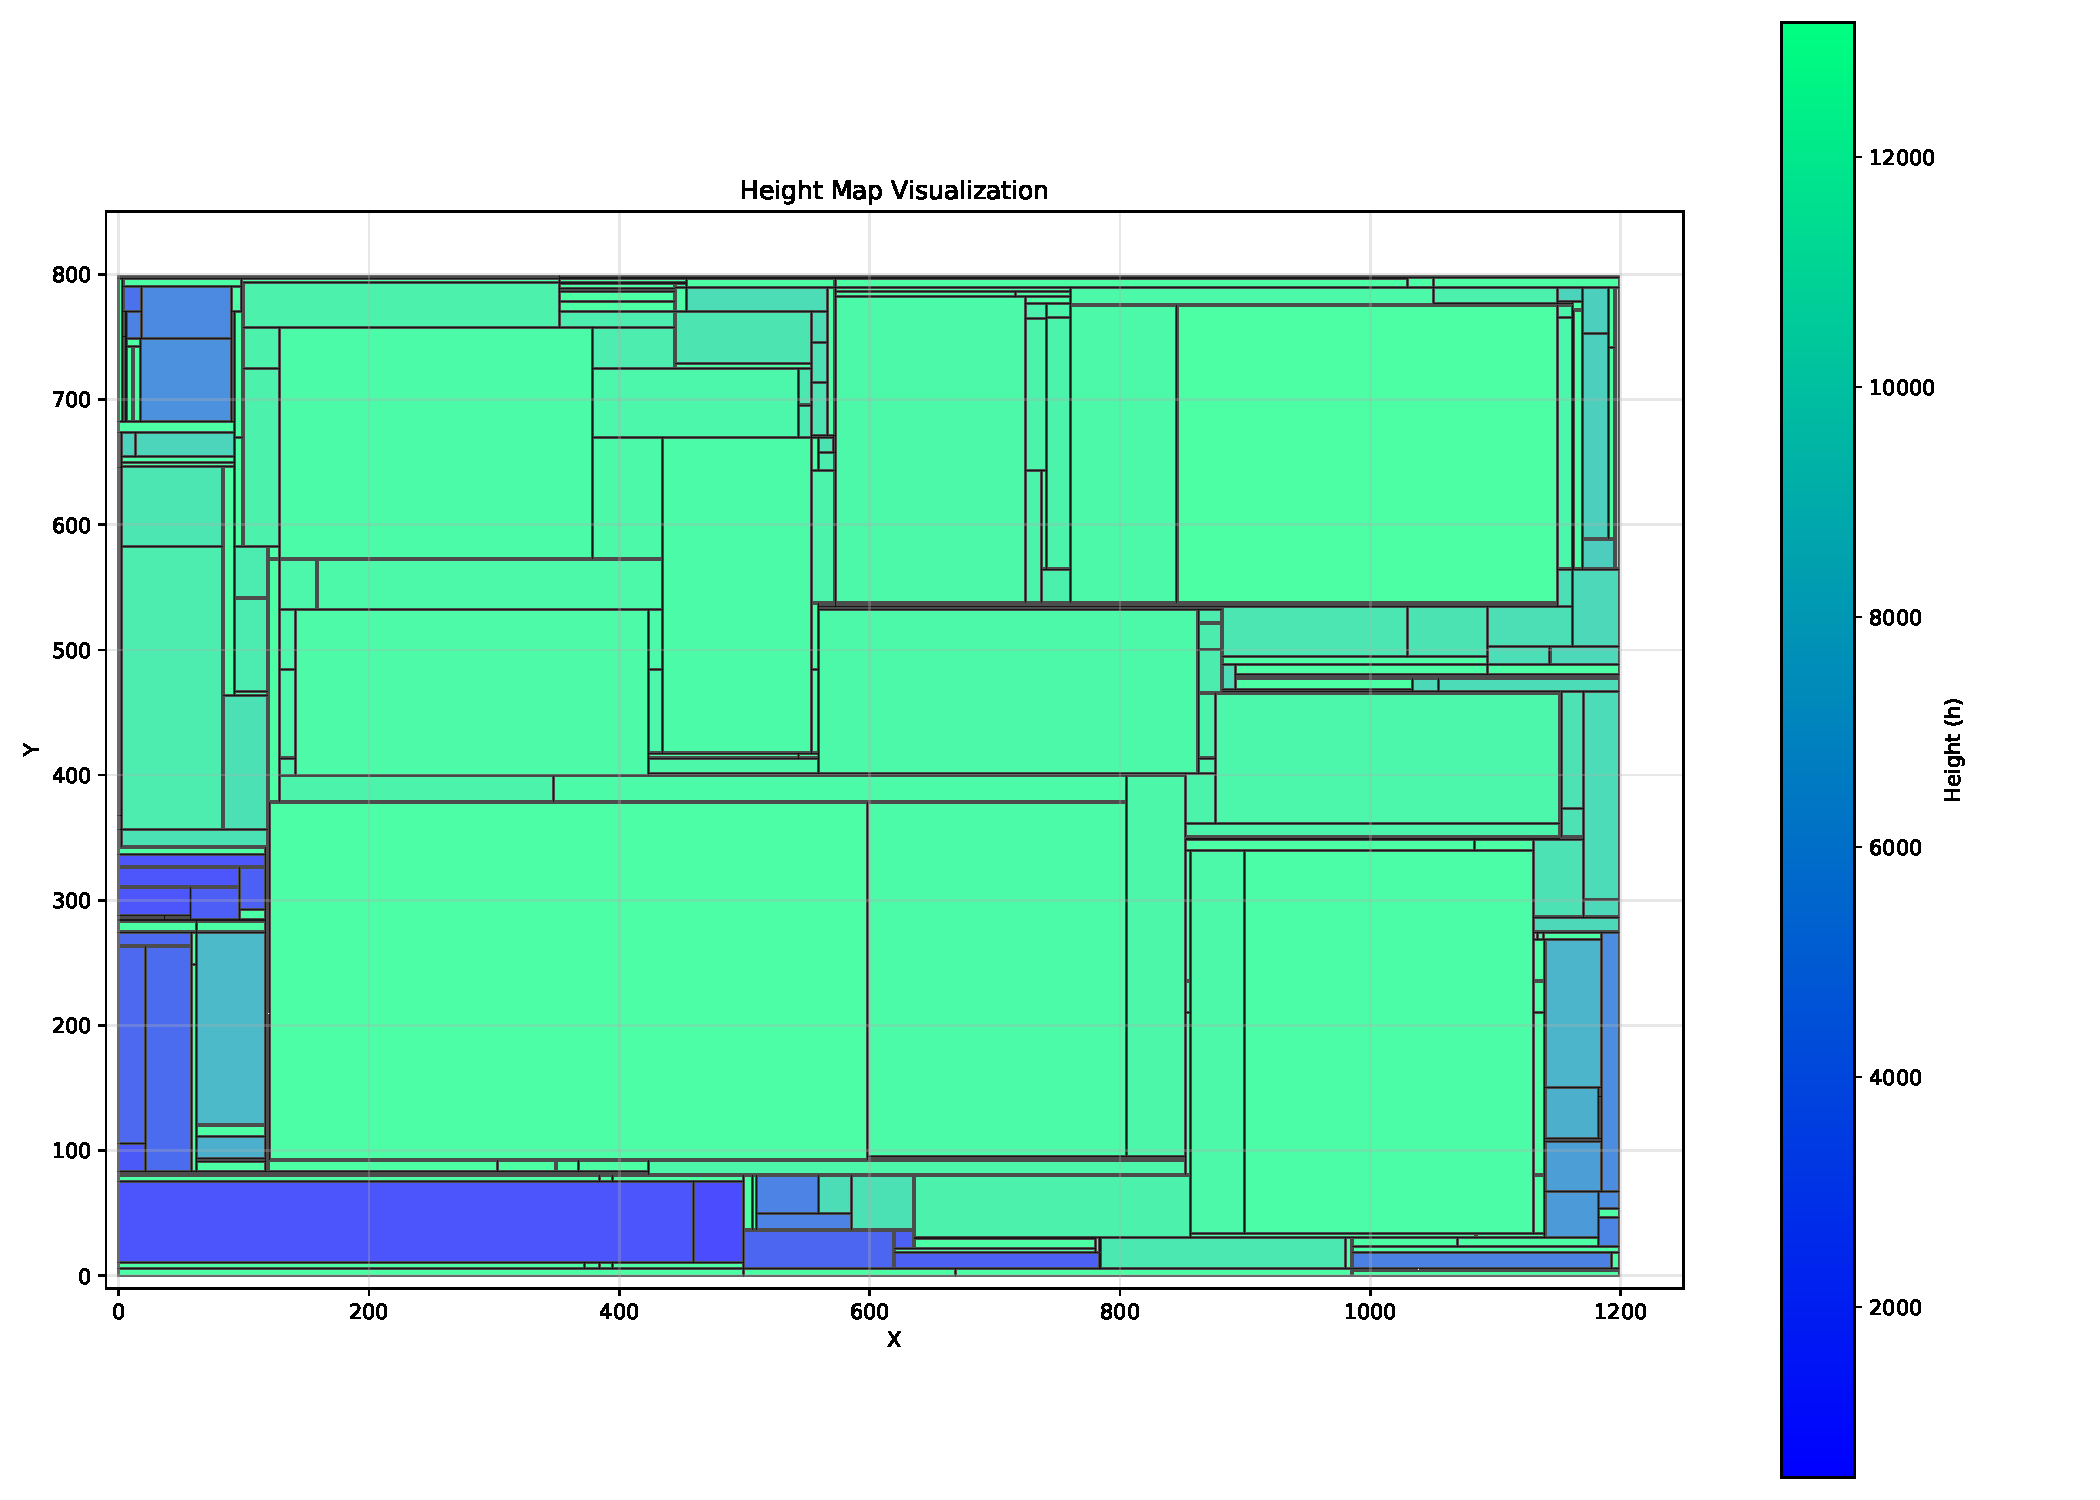
\includegraphics[width=1\textwidth]{figures/height_map.pdf}
\caption{Карта высот HeightHandler: вид сверху с цветовым кодированием высоты (синий --- низкие области, зелёный --- высокие)}
\label{fig:evyukh_height_map}
\end{figure}

Сравнительный анализ вычислительной сложности реализаций приведён в таблице~\ref{tab:evyukh_complexity}.

\begin{table}[H]
\centering
\caption{Сравнение вычислительной сложности реализаций HeightHandler}
\label{tab:evyukh_complexity}
\adjustbox{max width=\linewidth}{%
\begin{tabular}{|l|c|c|c|}
\hline
\textbf{Реализация} & $\mathtt{get\_h}$ & $\mathtt{get\_area}$ & $\mathtt{add\_rect}$ \\
\hline
Baseline & $O(n)$ & $O(n)$ & $O(1)$ \\
Rects & $O(n)$ & $O(n)$ & $O(n)$ \\
Grid & $O(k)$ & $O(k)$ & $O(k)$ \\
SegTree & $O(\log W \log H)$ & $O(\log W \log H)$ & $O(\log W \cdot H)$ \\
Quadtree & $O(\log(\max(W,H)))$ & $O(n)$ & $O(\log(\max(W,H)))$ \\
\hline
\end{tabular}}
\end{table}

Экспериментальное тестирование проводилось на 436 реальных задачах с суммарным количеством операций 27,5 миллионов. Результаты представлены в таблице~\ref{tab:evyukh_heighthandler}. Реализация Rects продемонстрировала наилучшую производительность. Данный результат объясняется эффективным использованием раннего выхода при сортировке по убыванию высоты, низкими накладными расходами простой структуры данных и эффективным использованием кэш-памяти процессора.

\begin{table}[H]
\centering
\caption{Результаты тестирования реализаций HeightHandler}
\label{tab:evyukh_heighthandler}
\begin{tabular}{|l|r|r|r|r|}
\hline
\textbf{Реализация} & \textbf{Всего, мс} & $\mathtt{get\_h}$, мс & $\mathtt{get\_area}$, мс & $\mathtt{add\_rect}$, мс \\
\hline
Baseline & 36412 & 19724 & 21231 & 4 \\
Rects & 1658 & 1713 & 2121 & 14 \\
Grid & 120688 & 32015 & 93547 & 112 \\
SegTree & 71199 & 34877 & 33292 & 5825 \\
Quadtree & 168971 & 86822 & 81857 & 885 \\
\hline
\end{tabular}
\end{table}

Реализации Grid, SegTree и Quadtree оказались медленнее базовой реализации. Причинами являются высокие накладные расходы на управление структурами данных, а также тот факт, что типичные коробки покрывают значительную часть паллеты, что нивелирует преимущества иерархических структур. В финальной версии алгоритма используется реализация Rects.

\section{Ограничение на устойчивость размещения}
\label{sec:stability_constraint}

Для обеспечения устойчивости укладки введено ограничение: коробка может быть размещена в позиции $(x, y)$ только в том случае, если центр масс основания коробки опирается на нижележащую коробку или на поверхность паллеты. Формально, если точка $(x + \frac{length}{2}, y + \frac{width}{2})$ находится на высоте $h$, то высота поверхности в этой точке также должна быть равна $h$.

Данное ограничение пассивно увеличивает минимальный коэффициент опоры (min\_support\_ratio) до значений порядка 0,25--0,30, поскольку коробки не могут <<висеть>> над пустотой. Без этого ограничения минимальный коэффициент опоры может падать до 0,01--0,03.

\section{Жадный алгоритм укладки}

Разработанный жадный алгоритм GreedySolver реализует последовательный подход к укладке коробок. Алгоритм обрабатывает коробки в порядке их появления во входных данных, выбирая для каждой коробки позицию с минимальной итоговой высотой.

На каждом шаге алгоритм получает очередную коробку из входного списка и рассматривает допустимые ориентации данной коробки. Поскольку коробки могут вращаться только вокруг вертикальной оси, допускается перестановка длины и ширины основания (length и width), что даёт две возможные ориентации для несимметричных коробок. Для каждой ориентации структура HeightHandler возвращает множество потенциальных позиций размещения. Позиции, не удовлетворяющие ограничению на устойчивость, отфильтровываются. Для оставшихся позиций вычисляется оценка качества как сумма текущей высоты поверхности и высоты размещаемой коробки. Выбирается позиция с минимальной оценкой, после чего коробка размещается и структура HeightHandler обновляется.

Псевдокод жадного алгоритма представлен в алгоритме~\ref{alg:evyukh_greedy}. Вычислительная сложность алгоритма составляет $O(n \cdot k \cdot m)$, где $n$ --- количество коробок, $k$ --- количество рассматриваемых ориентаций (не более 2), $m$ --- количество потенциальных позиций размещения.

\begin{algorithm}[H]
\caption{Жадный алгоритм укладки (GreedySolver)}
\label{alg:evyukh_greedy}
\KwIn{$boxes$ -- list of boxes, $pallet$ -- pallet dimensions}
\KwOut{$answer$ -- placement positions for all boxes}
$heightHandler \leftarrow$ create height map structure\;
\ForEach{$box \in boxes$}{
    $bestScore \leftarrow \infty$\;
    \ForEach{$rotatedBox \in getRotations(box)$}{
        \ForEach{$(x, y) \in heightHandler.getDots(rotatedBox)$}{
            \If{not isCenterOfMassSupported($x$, $y$, $rotatedBox$)}{
                continue\;
            }
            $h \leftarrow heightHandler.getH(x, y, x + rotatedBox.length, y + rotatedBox.width)$\;
            $score \leftarrow h + rotatedBox.height$\;
            \If{$score < bestScore$}{
                save best position $(x, y, h)$ and rotation\;
            }
        }
    }
    add box to $answer$ at best position\;
    $heightHandler.addRect(bestPosition, box.height)$\;
}
\Return{$answer$}
\end{algorithm}

\section{Алгоритм DBLF (Deepest Bottom Left Fill)}

Алгоритм DBLFSolver реализует стратегию Deepest Bottom Left Fill~\cite{karabulut}, отличающуюся от жадного алгоритма критерием выбора позиции. Вместо минимизации итоговой высоты $h_0 + h_{box}$ алгоритм DBLF минимизирует лексикографически кортеж $(h_0,\; x,\; y,\; h_0 + h_{box})$, где $h_0$ --- высота основания в точке размещения. Такой критерий обеспечивает размещение коробок как можно глубже (ниже), а при равной глубине --- как можно ближе к нижнему левому углу паллеты.

В отличие от GreedySolver, алгоритм DBLF не проверяет ограничение на устойчивость (поддержку центра масс), что позволяет достигать более высокого коэффициента заполнения, но приводит к крайне низкому минимальному коэффициенту опоры. Остальные элементы алгоритма (перебор ориентаций, использование HeightHandler) аналогичны жадному алгоритму. Вычислительная сложность составляет $O(n \cdot k \cdot m)$.

\section{Алгоритм FFD (First Fit Decreasing)}

Алгоритм FFDSolver реализует классическую стратегию First Fit Decreasing~\cite{CoffmanFFD1996}, при которой коробки предварительно сортируются по убыванию объёма $V = l \times w \times h$. После сортировки применяется тот же подход размещения, что и в GreedySolver: на каждом шаге выбирается позиция с минимальной итоговой высотой.

Предварительная сортировка по объёму обеспечивает размещение крупных коробок первыми, что позволяет сформировать более плотное основание паллеты. Аналогично алгоритму DBLF, FFDSolver не проверяет ограничение на устойчивость. Вычислительная сложность алгоритма составляет $O(n \log n + n \cdot k \cdot m)$, где первое слагаемое обусловлено сортировкой.

\section{Метаэвристический алгоритм на основе поиска в большой окрестности}

Для повышения качества укладки разработан метаэвристический алгоритм LNSSolver, основанный на методе поиска в большой окрестности (Large Neighborhood Search, LNS)~\cite{Pisinger2005}. Данный метод итеративно модифицирует текущее решение с помощью операторов мутации и принимает улучшающие изменения.

Решение кодируется классом GenomHandler (порядок коробок по паллетам и порог минимальной опоры). Каждый элемент массива содержит идентификатор коробки, выбранную ориентацию ($-1$ означает перебор всех) и предпочтительный угол паллеты для размещения. Порядок элементов в массиве определяет порядок укладки коробок: перестановка элементов приводит к другому варианту укладки.

Функция симуляции принимает закодированное решение и выполняет укладку согласно жадному алгоритму с учётом заданных параметров. Для каждой коробки рассматриваются указанные ориентации, формируется множество потенциальных позиций, выполняется фильтрация позиций по ограничению на устойчивость и по порогу минимальной опоры, и выбирается позиция с минимальной итоговой высотой. При равных высотах выбирается позиция ближе к предпочтительному углу. Результатом симуляции является укладка и набор метрик качества.

Для исследования пространства решений реализовано тринадцать операторов мутации. Операторы изменения порядка включают реверс подмассива, случайную перестановку, обмен двух элементов и обмен соседних элементов. Операторы сортировки упорядочивают коробки по площади основания, объёму, высоте или весу. Операторы изменения параметров модифицируют ориентации и предпочтительные углы размещения. Специальные операторы включают изменение порога минимальной опоры, группировку коробок одного типа и перемещение коробки с наименьшей опорой в начало последовательности.

Псевдокод алгоритма LNSSolver представлен в алгоритме~\ref{alg:evyukh_lns}. На каждой итерации выбирается случайный оператор мутации, применяется к копии текущего решения, и выполняется симуляция. Если новое решение улучшает целевую функцию, оно принимается как текущее.

\begin{algorithm}[H]
\caption{Алгоритм поиска в большой окрестности (LNSSolver)}
\label{alg:evyukh_lns}
\KwIn{$testData$ -- problem data, $timeLimit$ -- time limit}
\KwOut{$bestAnswer$ -- best found solution}
$params \leftarrow$ initialize with default order\;
$bestResult \leftarrow simulate(testData, params)$\;
\While{$currentTime < timeLimit$}{
    $newParams \leftarrow$ copy of $params$\;
    $mutation \leftarrow$ select random mutation operator\;
    apply $mutation$ to $newParams$\;
    $newResult \leftarrow simulate(testData, newParams)$\;
    \If{$newResult.score > bestResult.score$}{
        $bestResult \leftarrow newResult$\;
        $params \leftarrow newParams$\;
    }
}
\Return{$bestResult.answer$}
\end{algorithm}

Целевая функция вычисляется как взвешенная сумма метрик:
\[
\begin{split}
\text{score} = {}& w_1 \cdot \text{percolation}
    + w_2 \cdot \text{min\_support\_ratio} \\
&{}+ w_3 \cdot (1 - \text{CoM}_z^{\text{rel}})
    + w_4 \cdot \text{height\_balance},
\end{split}
\]
где $w_1, \ldots, w_4$ --- настраиваемые веса, $\text{CoM}_z^{\text{rel}}$ --- нормализованная $z$-координата центра масс, $\text{height\_balance}$ --- баланс высот между паллетами (см. раздел~\ref{sec:evyukh_multipallet}). Для задач с одной паллетой используются только первые два слагаемых ($w_3 = w_4 = 0$). Алгоритм использует критерий принятия только улучшений (hill-climbing): новое решение принимается только в случае улучшения значения целевой функции.

Важной оптимизацией LNSSolver является выборочный пересчёт: после применения мутации пересчитываются только те паллеты, содержимое которых было изменено. Это достигается с помощью маски <<грязных>> паллет (pallet\_dirty), что существенно ускоряет работу в мультипаллетном режиме.

\section{Генетический алгоритм}

Разработан генетический алгоритм GeneticSolver, использующий ту же модель кодирования решения (GenomHandler) и те же 13 операторов мутации, что и LNSSolver, но применяющий популяционный подход.

Алгоритм поддерживает популяцию из $P = 24$ особей. Начальная популяция формируется случайной перестановкой порядка коробок. На каждой итерации из лучших~8 особей популяции случайным образом выбирается родитель, к которому применяется оператор мутации, после чего выполняется полная симуляция укладки. Полученное потомство добавляется в новое поколение. Лучшая найденная особь всегда сохраняется (элитизм).

В отличие от LNSSolver, генетический алгоритм на каждой итерации пересчитывает все паллеты заново (вызов rebuild\_all), поскольку особи популяции независимы. Это приводит к тому, что GeneticSolver выполняет меньше итераций за единицу времени по сравнению с LNSSolver, особенно при большом числе паллет.

\section{Укладка на несколько паллет}
\label{sec:evyukh_multipallet}

Для обработки ситуаций, когда груз необходимо разместить на нескольких паллетах, алгоритмы обобщены на мультипаллетный режим. Количество доступных паллет задаётся параметром $P$, а коробки равномерно распределяются между паллетами.

В метаэвристических алгоритмах (LNSSolver и GeneticSolver) операторы мутации могут модифицировать как порядок коробок внутри одной паллеты, так и перемещать коробки между паллетами (оператор swap\_boxes\_across\_pallets).

Для оценки равномерности загрузки паллет введена метрика баланса высот:
\[
\text{height\_balance} = \max\Bigl(0,\; 1 - \frac{\sigma(H_1, \ldots, H_P)}{\mu(H_1, \ldots, H_P)}\Bigr).
\]
где $H_i$ --- высота штабеля на $i$-й паллете, $\sigma$ --- стандартное отклонение, $\mu$ --- среднее значение. Метрика принимает значение~1 при одинаковых высотах и стремится к~0 при сильном разбросе. Параметр $w_4$ в целевой функции управляет значимостью баланса высот при оптимизации.

\section{Результаты экспериментов}
\label{sec:evyukh_experiments}

Экспериментальное тестирование проводилось на наборе из 436 реальных задач. Размеры паллеты составляли $1200 \times 800$ мм.
На рисунке~\ref{fig:evyukh_pallet_example} представлен пример построенной паллеты, демонстрирующий качество укладки, достигаемое разработанным алгоритмом LNSSolver. Укладка характеризуется плотным заполнением пространства и устойчивым размещением коробок.

\begin{figure}[H]
\centering
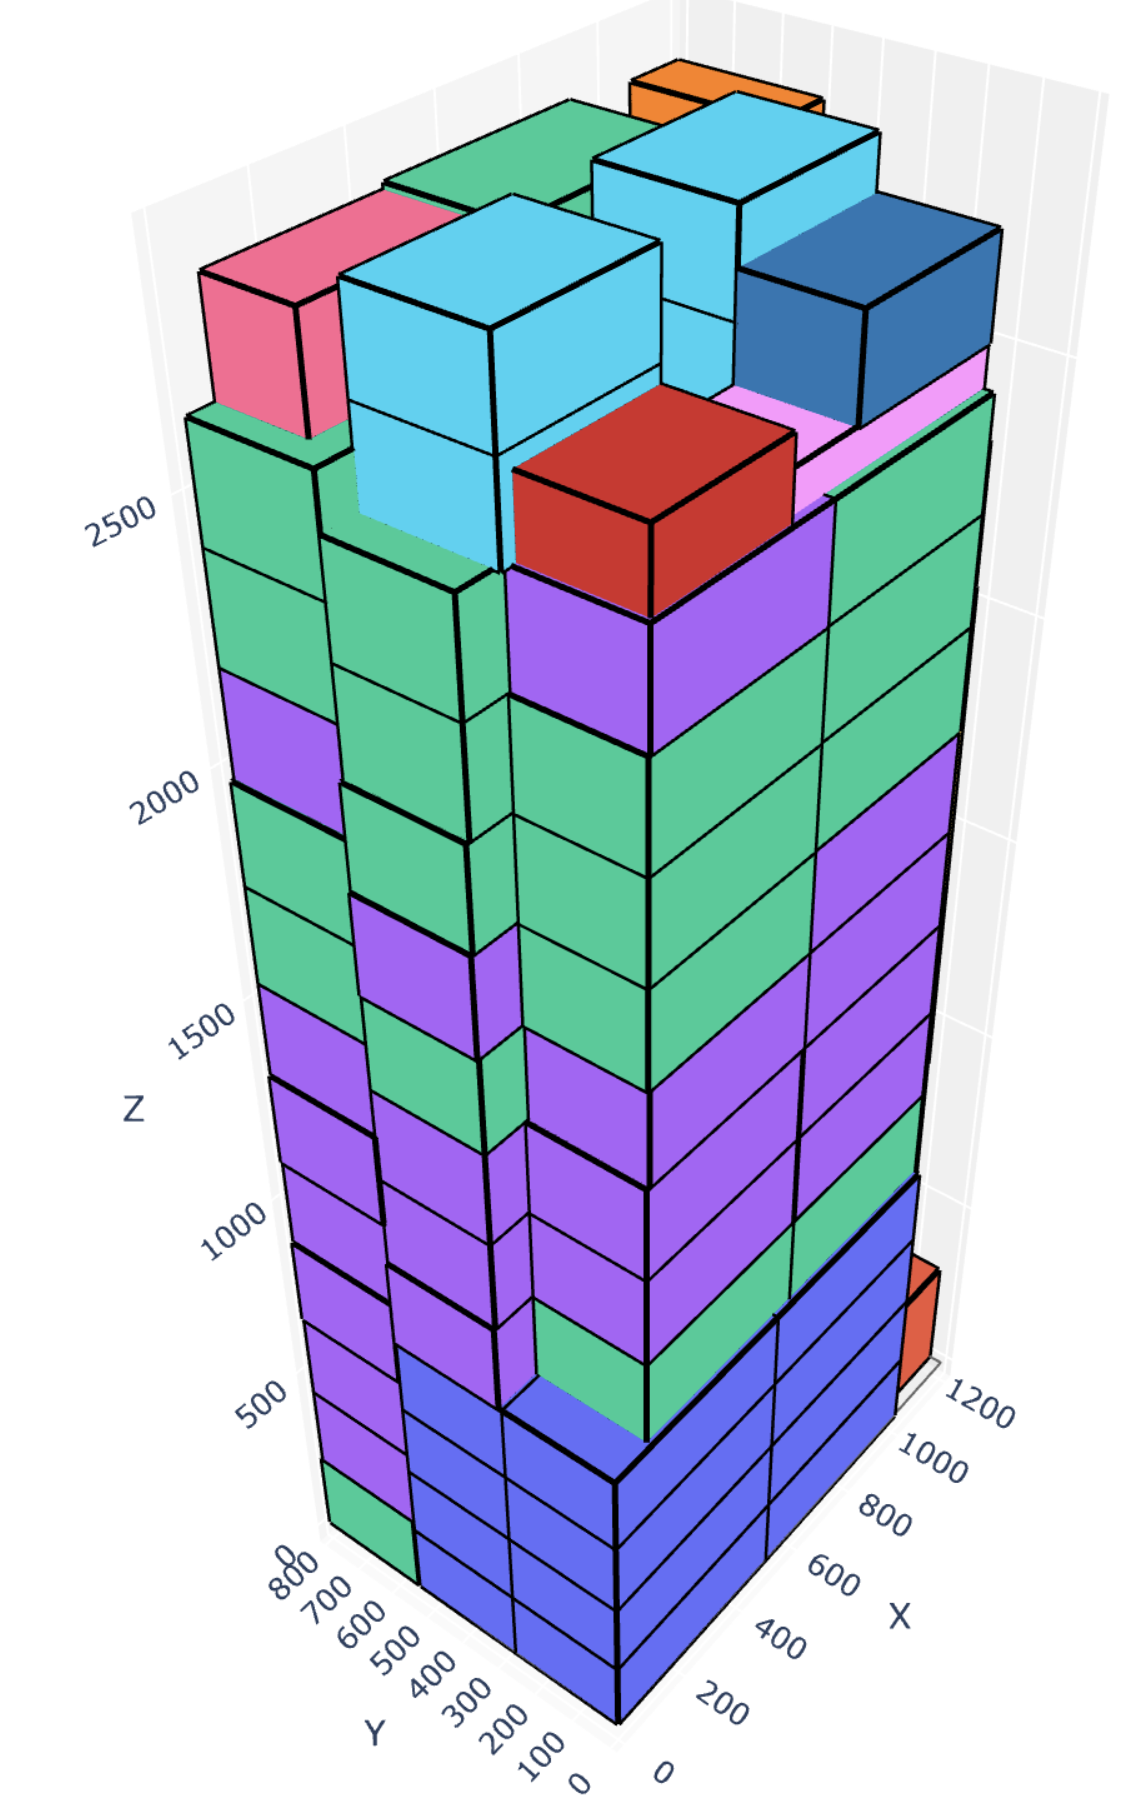
\includegraphics[width=0.7\textwidth]{figures/eyu_test_153.png}
\caption{Пример построенной паллеты: трёхмерная визуализация результата работы алгоритма LNSSolver}
\label{fig:evyukh_pallet_example}
\end{figure}

Видеозапись процесса симуляции укладки паллеты, демонстрирующая последовательное размещение коробок сверху вниз, доступна по ссылке: \url{https://disk.360.yandex.ru/d/xRs8nw0dt8-esw}.

Исходный код разработанного программного решения размещён в открытом репозитории: \url{https://github.com/Straple/Palletizer}.


На рисунке~\ref{fig:evyukh_weights} представлена зависимость качества укладки от веса $w_2$ при фиксированном $w_1 = 1{,}0$ и временном лимите 10 секунд. Видно, что увеличение веса $w_2$ приводит к росту минимального коэффициента опоры с 28\% до 69\%, однако при этом коэффициент заполнения снижается с 71\% до 63\%. Значение $w_2 = 2{,}0$ обеспечивает баланс между заполнением и устойчивостью.

\begin{figure}[H]
\centering
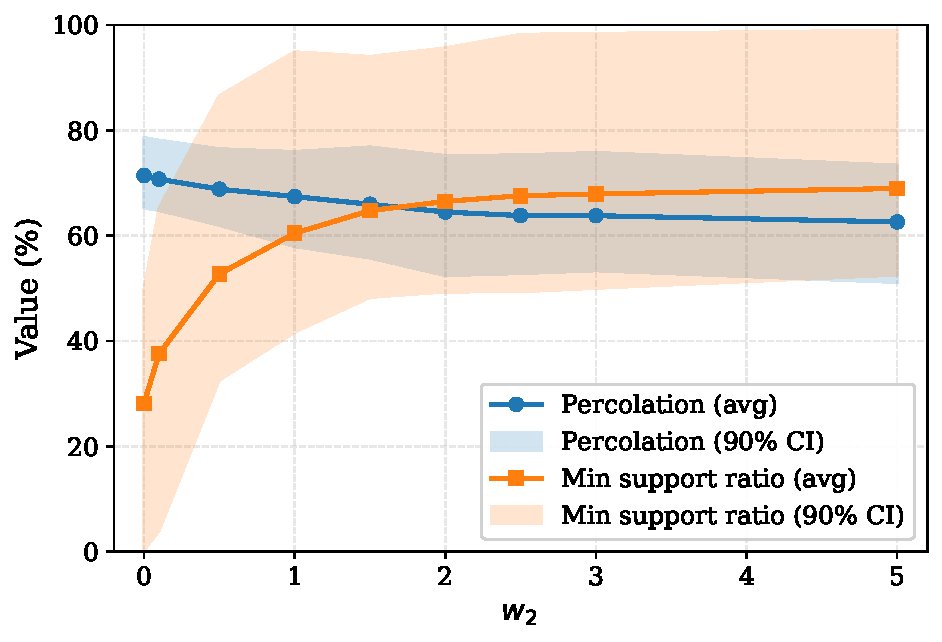
\includegraphics[width=\textwidth]{figures/weights_comparison.pdf}
\caption{Зависимость качества укладки от веса $w_2$ (время = 10с, $w_1=1$)}
\label{fig:evyukh_weights}
\end{figure}

На рисунке~\ref{fig:evyukh_time} представлена зависимость качества укладки от временного лимита при фиксированных весах $w_1 = 1{,}0$, $w_2 = 2{,}0$. С увеличением времени выполнения с 0,5 до 60 секунд коэффициент заполнения возрастает с 56\% до 67\%, а минимальный коэффициент опоры --- с 59\% до 69\%.

\begin{figure}[H]
\centering
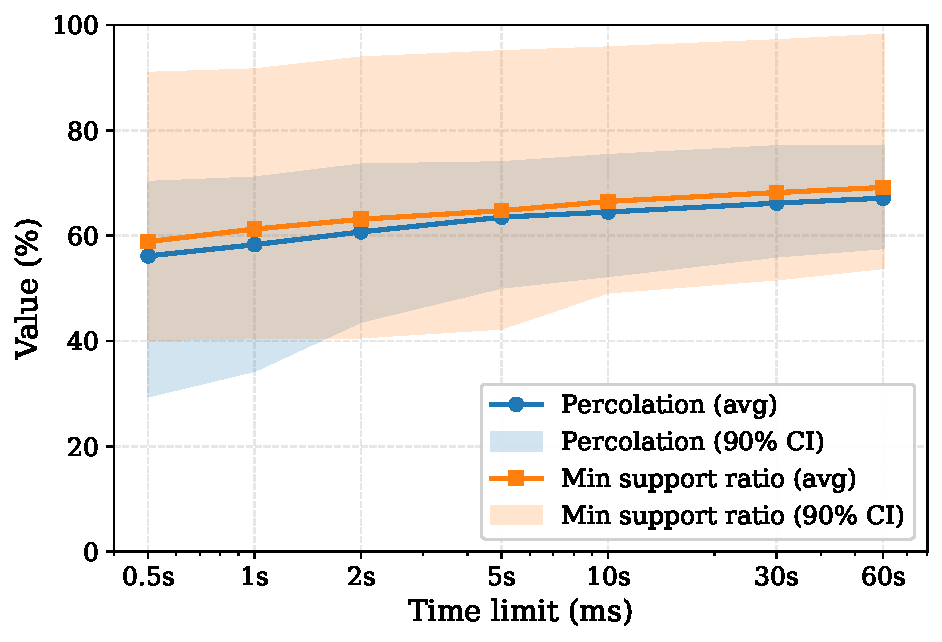
\includegraphics[width=\textwidth]{figures/time_comparison.pdf}
\caption{Зависимость качества укладки от времени выполнения ($w_1=1$, $w_2=2$)}
\label{fig:evyukh_time}
\end{figure}

Для оценки влияния ограничения на устойчивость было проведено сравнение алгоритма LNSSolver с включённым и отключённым ограничением (таблица~\ref{tab:evyukh_stability}). В штатном режиме со включённым ограничением средняя перколяция составляет 71,42\%, минимальный коэффициент опоры --- 28,16\%. При отключении ограничения коэффициент заполнения возрастает до 76,69\%, однако минимальный коэффициент опоры падает до 2,86\%, что неприемлемо для практического применения.

\begin{table}[H]
\centering
\caption{Влияние ограничения на устойчивость (10 сек на тест, $w_1=1$, $w_2=0$)}
\label{tab:evyukh_stability}
\adjustbox{max width=\linewidth}{%
\begin{tabular}{|l|c|c|}
\hline
\textbf{Режим} & \textbf{Перколяция, \%} & \textbf{Мин. опора, \%} \\
\hline
С ограничением на устойчивость & 71,42\% & 28,16\% \\
Без ограничения на устойчивость & 76,69\% & 2,86\% \\
\hline
\end{tabular}}
\end{table}

Сравнение всех пяти разработанных алгоритмов на 436 реальных задачах с одной паллетой (лимит 5~с, $w_1 = 1{,}0$, $w_2 = 2{,}0$) приведено в таблице~\ref{tab:evyukh_all_solvers}.

\begin{table}[H]
\centering
\caption{Сравнение алгоритмов при одной паллете (436~тестов, 5~с)}
\label{tab:evyukh_all_solvers}
\adjustbox{max width=\linewidth}{%
\small
\setlength{\tabcolsep}{3pt}%
\begin{tabular}{|l|c|c|c|c|}
\hline
\textbf{Алгоритм} & \textbf{Перколяция, \%} & \textbf{Мин. опора, \%} & \textbf{Устойчивость} & \textbf{Время, мс} \\
\hline
GreedySolver   & 56,04 & 30,31 & да  &    12,8 \\
DBLFSolver     & 65,19 &  2,44 & нет &     7,5 \\
FFDSolver      & 66,36 &  2,46 & нет &     8,3 \\
GeneticSolver  & 63,45 & 62,02 & да  & 5130,6 \\
LNSSolver      & 63,49 & 64,74 & да  & 5008,5 \\
\hline
\end{tabular}%
}
\end{table}

На рисунке~\ref{fig:evyukh_algo_comparison} наглядно представлено сравнение алгоритмов с 90\%-ными доверительными интервалами.

\begin{figure}[H]
\centering
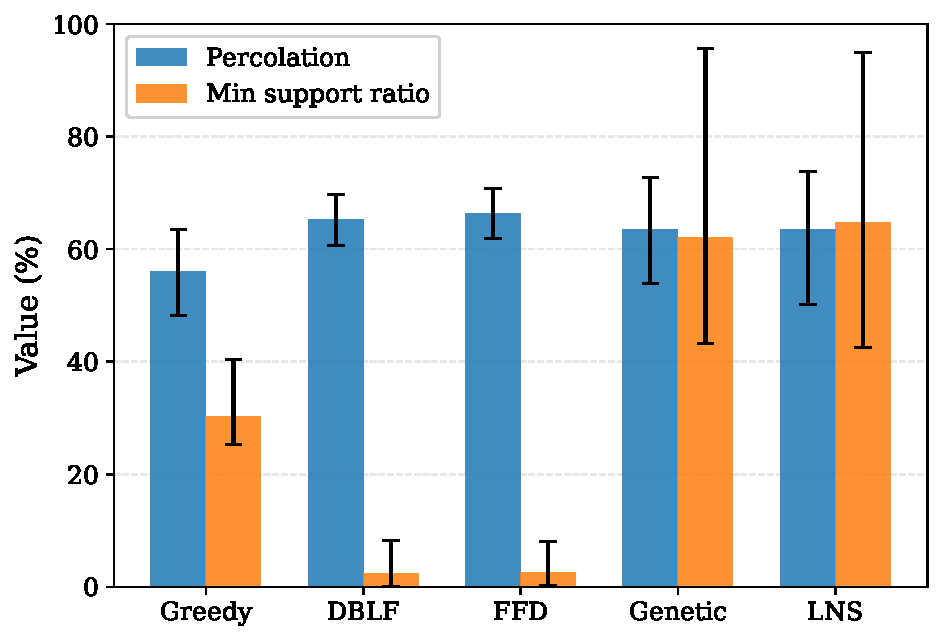
\includegraphics[width=\textwidth]{figures/algorithm_comparison.pdf}
\caption{Сравнение алгоритмов: перколяция и минимальный коэффициент опоры (одна паллета, 5~с)}
\label{fig:evyukh_algo_comparison}
\end{figure}

Результаты позволяют выделить две группы алгоритмов. Детерминированные эвристики (DBLFSolver, FFDSolver) достигают наилучшего коэффициента заполнения (65--66\%) при времени выполнения менее 10 мс, однако минимальный коэффициент опоры составляет лишь 2,4\%, что неприемлемо для практического применения. Низкая устойчивость обусловлена отсутствием проверки ограничения на поддержку центра масс.

У LNSSolver и GeneticSolver близкие значения перколяции (около 63,5\%), но у LNSSolver выше минимальный коэффициент опоры: 64,74\% против 62,02\%. В реализации LNS пересчитывается не вся конфигурация целиком, за счёт чего за то же время удаётся выполнить больше итераций поиска.

GreedySolver даёт 56,04\% перколяции и 30,31\% минимальной опоры; среди эвристик с учётом устойчивости он самый быстрый (12,8~мс).

\section{Сравнение LNSSolver и GeneticSolver при различных временных лимитах}

На рисунке~\ref{fig:evyukh_lns_vs_genetic} --- перколяция и минимальная опора обоих алгоритмов в зависимости от лимита времени.

\begin{figure}[H]
\centering
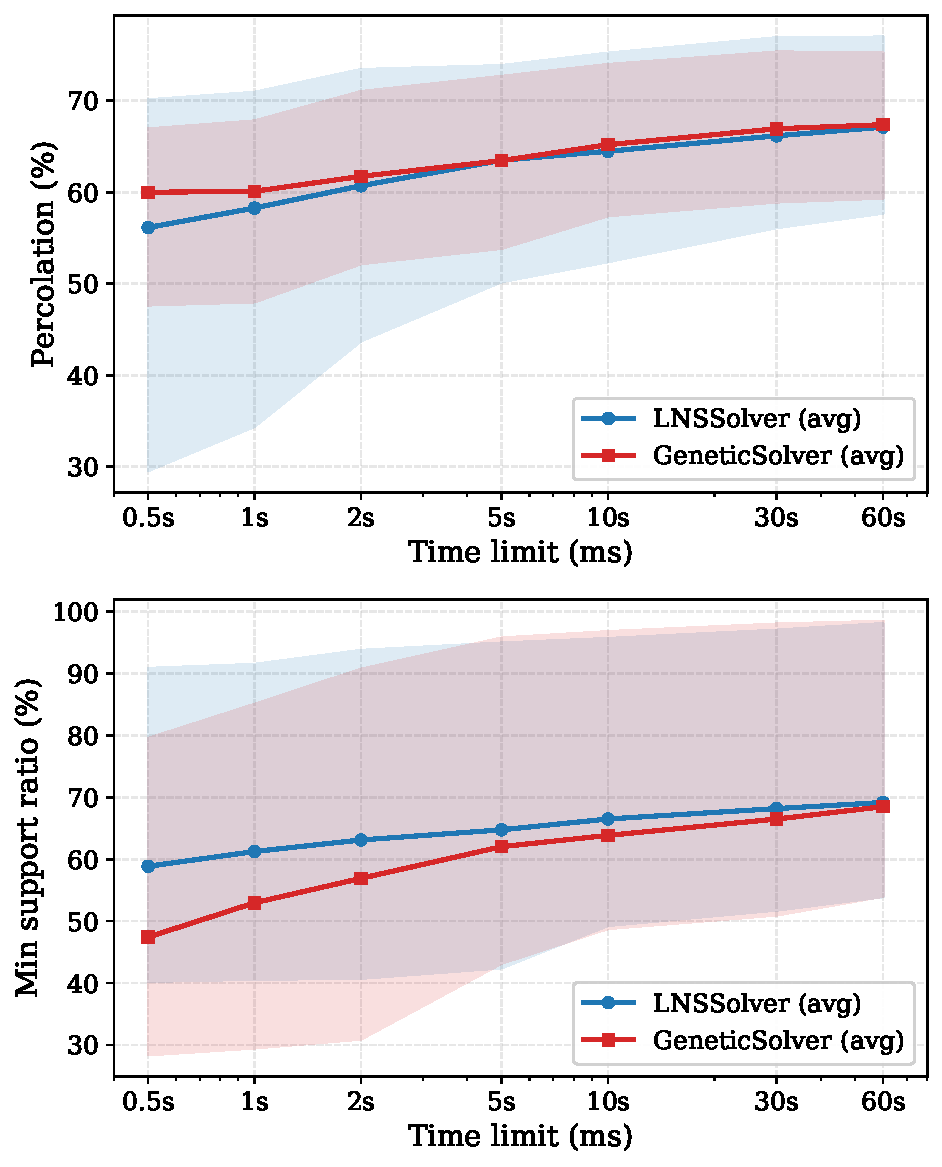
\includegraphics[width=\textwidth]{figures/lns_vs_genetic_time.pdf}
\caption{Сравнение LNSSolver и GeneticSolver: перколяция и минимальный коэффициент опоры при различных временных лимитах}
\label{fig:evyukh_lns_vs_genetic}
\end{figure}

При лимите 0,5--2~с у LNSSolver заметно выше минимальная опора; при росте лимита до 60~с отличия сглаживаются, GeneticSolver подтягивается по качеству. На коротких интервалах у генетического алгоритма иногда выигрывает перколяция: популяция стартовых решений даёт более широкий охват пространства поиска.

\section{Результаты в мультипаллетном режиме}

Результаты в мультипаллетном режиме при тех же условиях (лимит 5~с, $w_1 = 1{,}0$, $w_2 = 2{,}0$) приведены в таблице~\ref{tab:evyukh_multi}.

\begin{table}[H]
\centering
\caption{Сравнение алгоритмов в мультипаллетном режиме (лимит 5~с)}
\label{tab:evyukh_multi}
\adjustbox{max width=\linewidth}{%
\small
\setlength{\tabcolsep}{3pt}%
\begin{tabular}{|l|c|c|c|c|}
\hline
\textbf{Алгоритм} & \textbf{Перколяция, \%} & \textbf{Мин. опора, \%} & \textbf{Баланс высот, \%} & \textbf{Время, мс} \\
\hline
GreedySolver   & 55,33 & 19,08 & 83,57 &   38,2 \\
DBLFSolver     & 64,60 &  0,44 & 85,36 &   21,2 \\
FFDSolver      & 65,22 &  0,42 & 52,16 &   20,9 \\
GeneticSolver  & 59,01 & 44,06 & 84,83 & 5470,6 \\
LNSSolver      & 62,09 & 42,30 & 84,26 & 5016,7 \\
\hline
\end{tabular}%
}
\end{table}

В мультипаллетном режиме FFDSolver демонстрирует критически низкий баланс высот (52,16\%), поскольку при сортировке по объёму крупные коробки концентрируются на первых паллетах. Алгоритмы с метаэвристической оптимизацией обеспечивают баланс высот на уровне 84--85\%. LNSSolver сохраняет лидерство по коэффициенту заполнения среди метаэвристик (62,09\% против 59,01\% у GeneticSolver) благодаря оптимизации выборочного пересчёта паллет.

\section{Влияние веса баланса высот в мультипаллетном режиме}

На рисунке~\ref{fig:evyukh_hb_sweep} представлена зависимость метрик качества от веса $w_4$ (баланс высот) при фиксированных $w_1 = 1{,}0$, $w_2 = 2{,}0$ и временном лимите 10~с.

\begin{figure}[H]
\centering
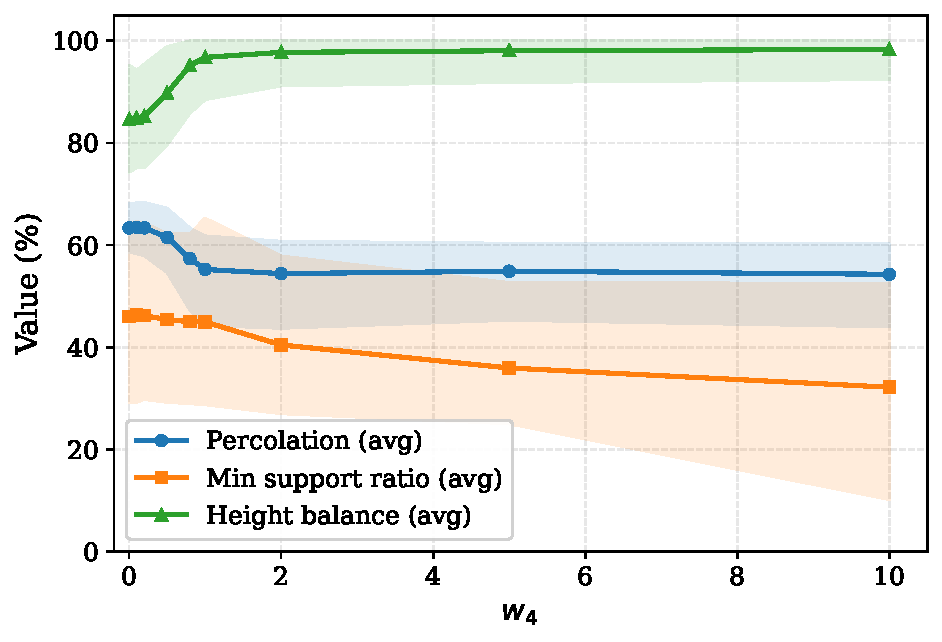
\includegraphics[width=\textwidth]{figures/height_balance_sweep.pdf}
\caption{Зависимость метрик качества от веса $w_4$ в мультипаллетном режиме (LNSSolver, 10~с)}
\label{fig:evyukh_hb_sweep}
\end{figure}

Увеличение $w_4$ приводит к росту баланса высот с 85\% до 98\%, однако за счёт снижения перколяции (с 63\% до 54\%) и минимального коэффициента опоры (с 46\% до 32\%). Значения $w_4 \in [0{,}2;\; 1{,}0]$ обеспечивают оптимальный компромисс: баланс высот превышает 85\% при умеренном снижении остальных метрик.
